% ============================================================

\begin{frame}{Which Face, by Seat Type}
\hypertarget{src:seathet}{}
\small
Mayoral races split by whether the seat is open, meaning the incumbent is term-limited so no front-runner defends it ($N=2{,}026$), or contested, where the sitting mayor may still seek re-election ($N=3{,}534$). This split is what assigns the face. The margin widens in both, so only the ballot separates them.
\smallskip
\begin{center}
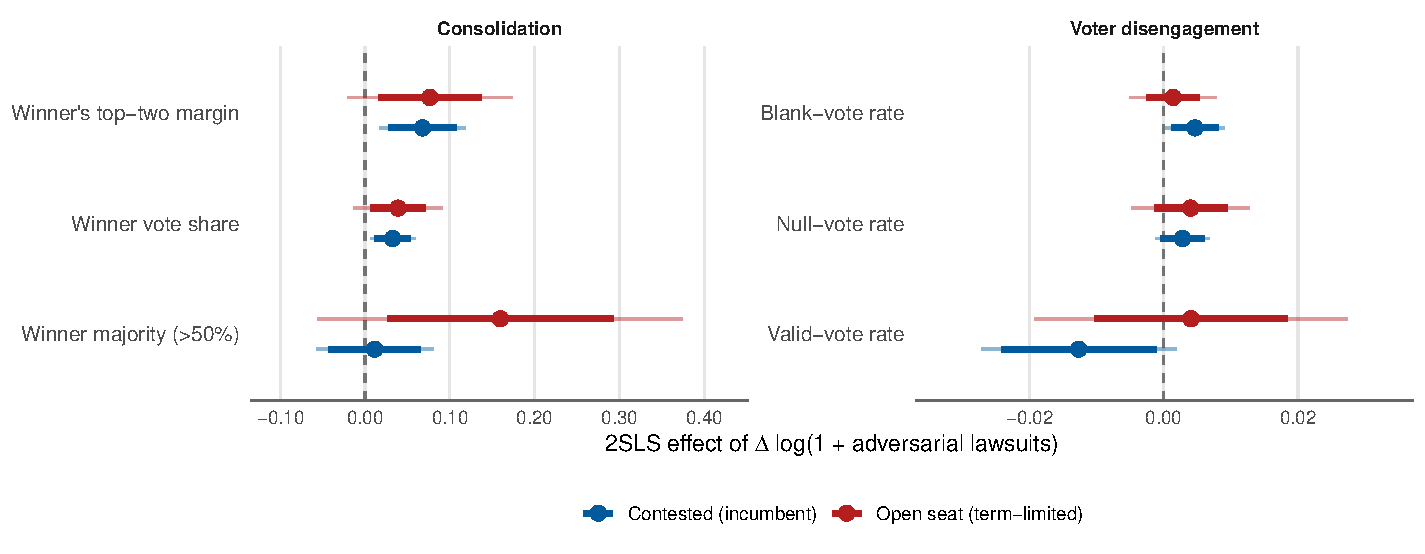
\includegraphics[width=\linewidth,height=0.44\textheight,keepaspectratio]{../figures/heterogeneity_seat_coefplot.pdf}
\end{center}
\smallskip
\takeaway{The winner's top-two margin widens in both seat types ($+0.076$, $p=.05$ open; $+0.068$, $p=.01$ contested), so the consolidation is general. The mechanism splits by seat. In open seats it is \pos{decisiveness}: the winner crosses 50\% ($+0.160$, $p=.06$) with no ballot demobilization. In contested seats it carries a \negt{barrier} signature: blank votes rise ($+0.005$, $p=.04$) and valid votes fall ($-0.013$, $p=.08$) as voters confront an entrenched incumbent, with no majority shift ($p=.74$). The same shock produces decisiveness where the seat is open and disengagement where it is defended.}\hfill\hyperlink{app:seathet}{\beamergotobutton{full table}}
\end{frame}
